\section{Experimental Setup}
Figure. \ref{fig:all_detector} and \ref{fig:all_detector_topview} show a schematic view and a CAD drawing of the entire set of detectors.
Central neutrino target detectors consist of two Wagasci modules and T2K INGRID proton module. 
Inside the Wagasci module, plastic scintillator bars are aligned as a 3D grid-like structure
and spaces in the structure are filled with water for a water-in Wagasci module.
T2K INGRID proton module is a full active neutrino target detector which is composed only with scintillator bars in its tracking region. 
% The Wagasci modules consist of 3D grid-structure plastic-scintillator detectors filled with water as the neutrino interaction target.
% A central detector, Wagasci modules, consists of 3D grid-structure plastic-scintillator detectors filled with water as the neutrino interaction target.
The central detectors are surrounded by two side- and one downstream- muon range detectors(MRD's)
The MRD's are used to select muon tracks from the charged-current (CC) interactions 
and to reject short tracks caused by neutral particles 
that originate mainly from neutrino interactions in material surrounding the central detector, like the walls of the detector hall,
neutrons and gammas, or neutral-current (NC) interactions.
The muon momentum can be reconstructed from its range inside the detector.
The MRD's consist of plastic scintillators and iron plates.
In addition, each of the iron plates of the downstream-MRD, so called the Baby MIND detector, is wound by a coil and
can be magnetized. It provide the charge selection capability.


For all detectors, scintillation light in the scintillator bar is collected and transported to a photodetector with a wavelength shifting fiber (WLS fiber).
The light is read out by a photodetector, Multi-Pixel Photon Counter (MPPC), attached to one end of the WLS fiber.
The signal from the MPPC is read out by the dedicated electronics developed for the test experiment
to enable bunch separation in the beam spill.
The readout electronics is triggered using the beam-timing signal from MR to synchronize to the beam.
The beam-timing signal is branched from those for T2K, and will not cause any effect on the T2K data taking.

\begin{figure}[tbh]
\begin{center}
\includegraphics[width=0.8\linewidth]{fig/wagasci_smrd_babymind.pdf}
% \includegraphics[width=0.8\linewidth]{fig/all_detector2.pdf}
\end{center}
\caption{
Schematic view of entire sets of detectors.
}
\label{fig:all_detector}
\end{figure}

\begin{figure}[tbh]
\begin{center}
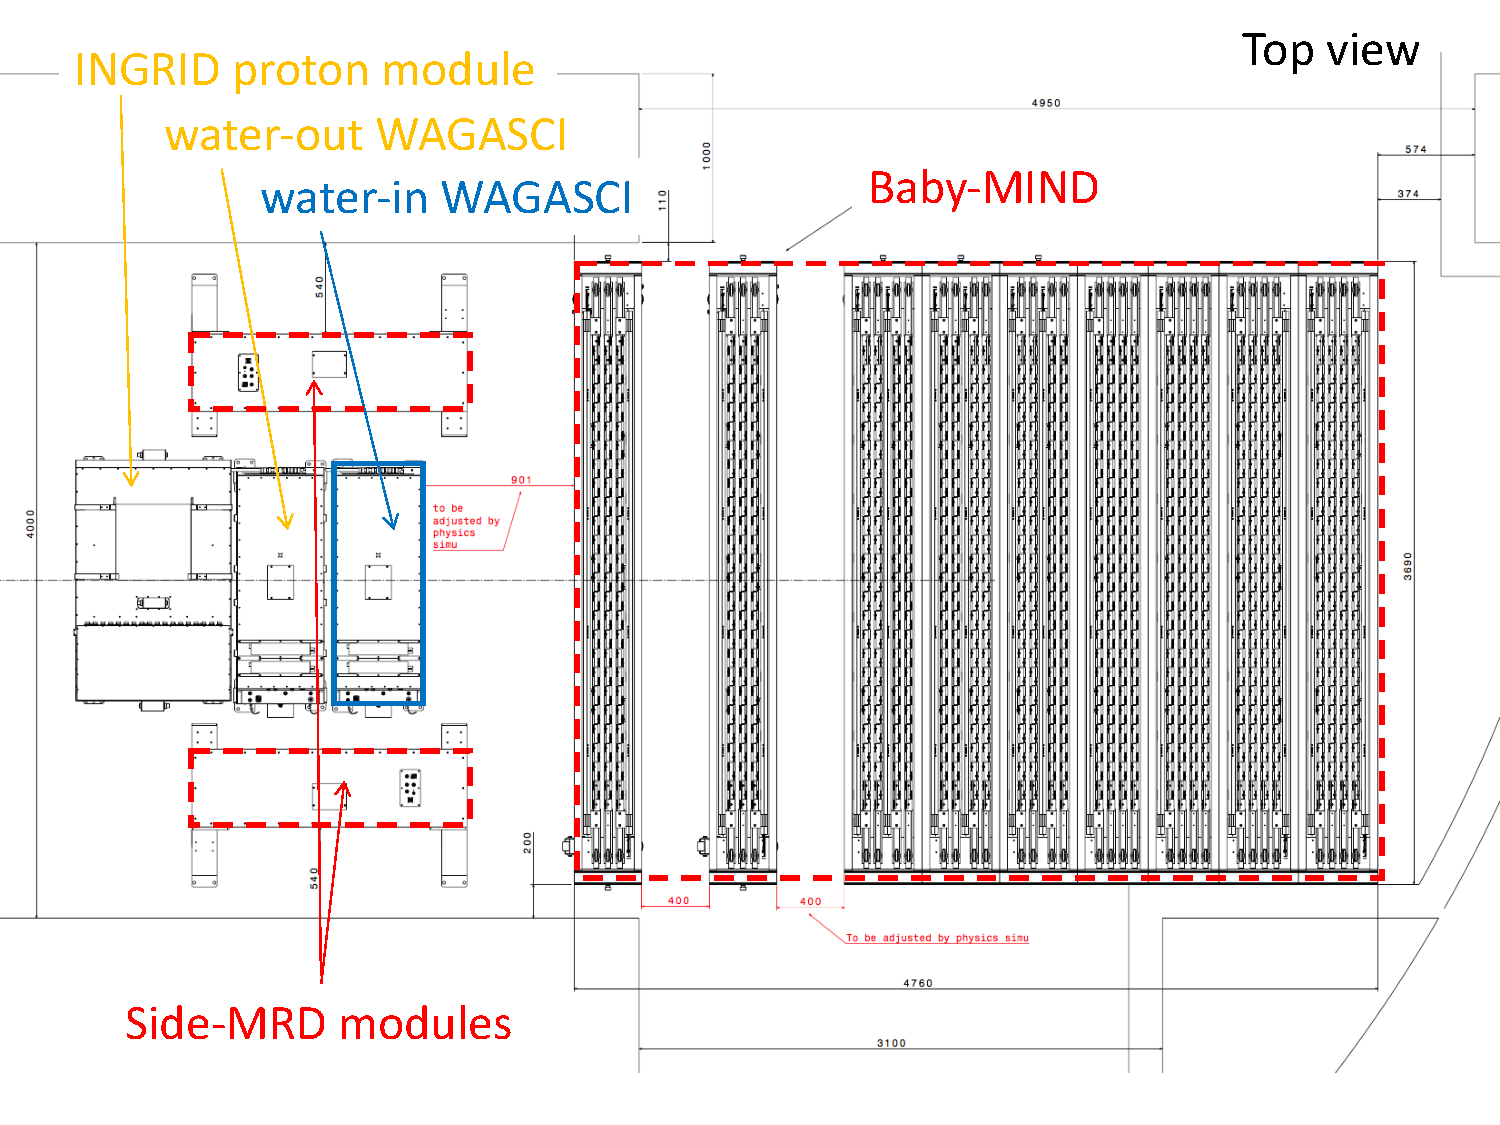
\includegraphics[width=0.8\linewidth]{fig/wagasci_smrd_babymind_topview.pdf}
% \includegraphics[width=0.8\linewidth]{fig/all_detector2.pdf}
\end{center}
\caption{
Top view of entire sets of detectors.
}
\label{fig:all_detector_topview}
\end{figure}


T2K adopted the off-axis beam method, in which
the neutrino beam is intentionally directed 2.5 degrees away from SK producing a narrow band $\nu_{\mu}$ beam.
The off-axis near detector, ND280, is installed towards the SK direction in the B1 floor of the near detector hall of the J-PARC neutrino beam-line.
We propose to install our detector in the B2 floor of the near detector hall, 
where the off-axis angle is similar but slightly different: 1.5 degree.
The candidate detector position in the B2 floor is shown in Fig. \ref{fig:location}.
The expected neutrino energy spectrum at the candidate position is shown in Fig. \ref{fig:b2flux}.

\begin{figure}[tbhp]
\begin{center}
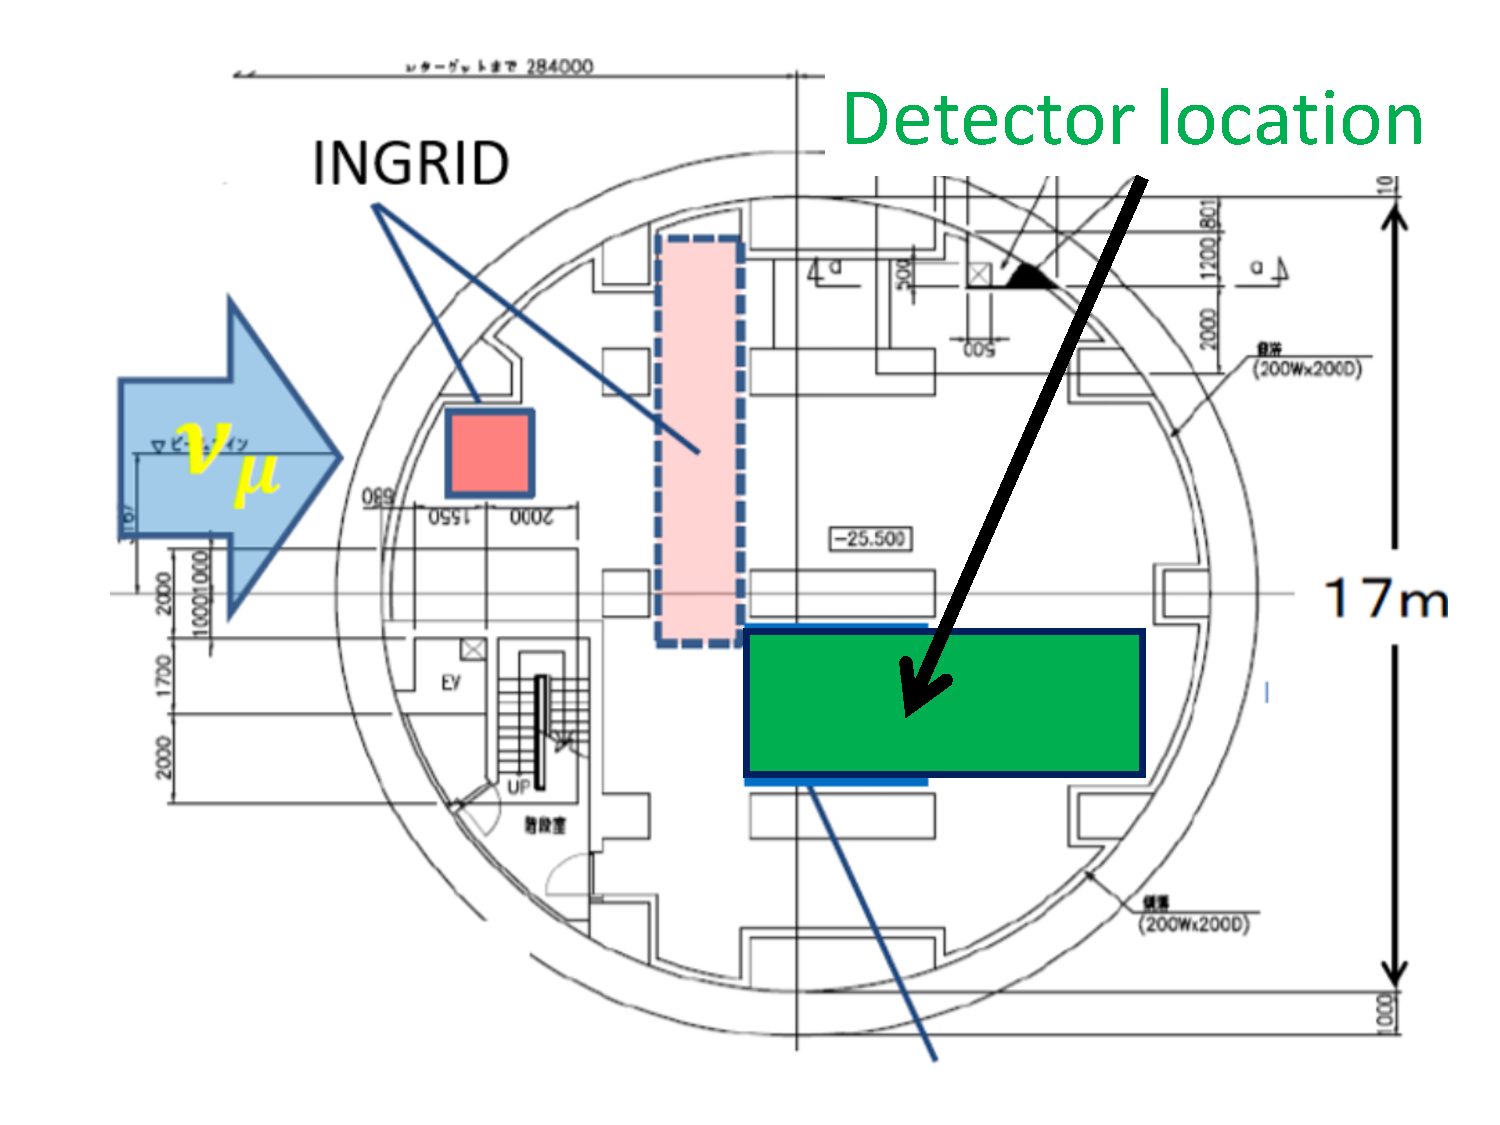
\includegraphics[width=0.6\linewidth]{fig/detector_position_b2.pdf}
% 
\includegraphics[width=0.6\linewidth]{fig/tmp.pdf}
\end{center}
\caption{
Candidate detector position in the B2 floor of the near detector hall.
}
\label{fig:location}
\end{figure}

\begin{figure}[tbhp]
\begin{center}
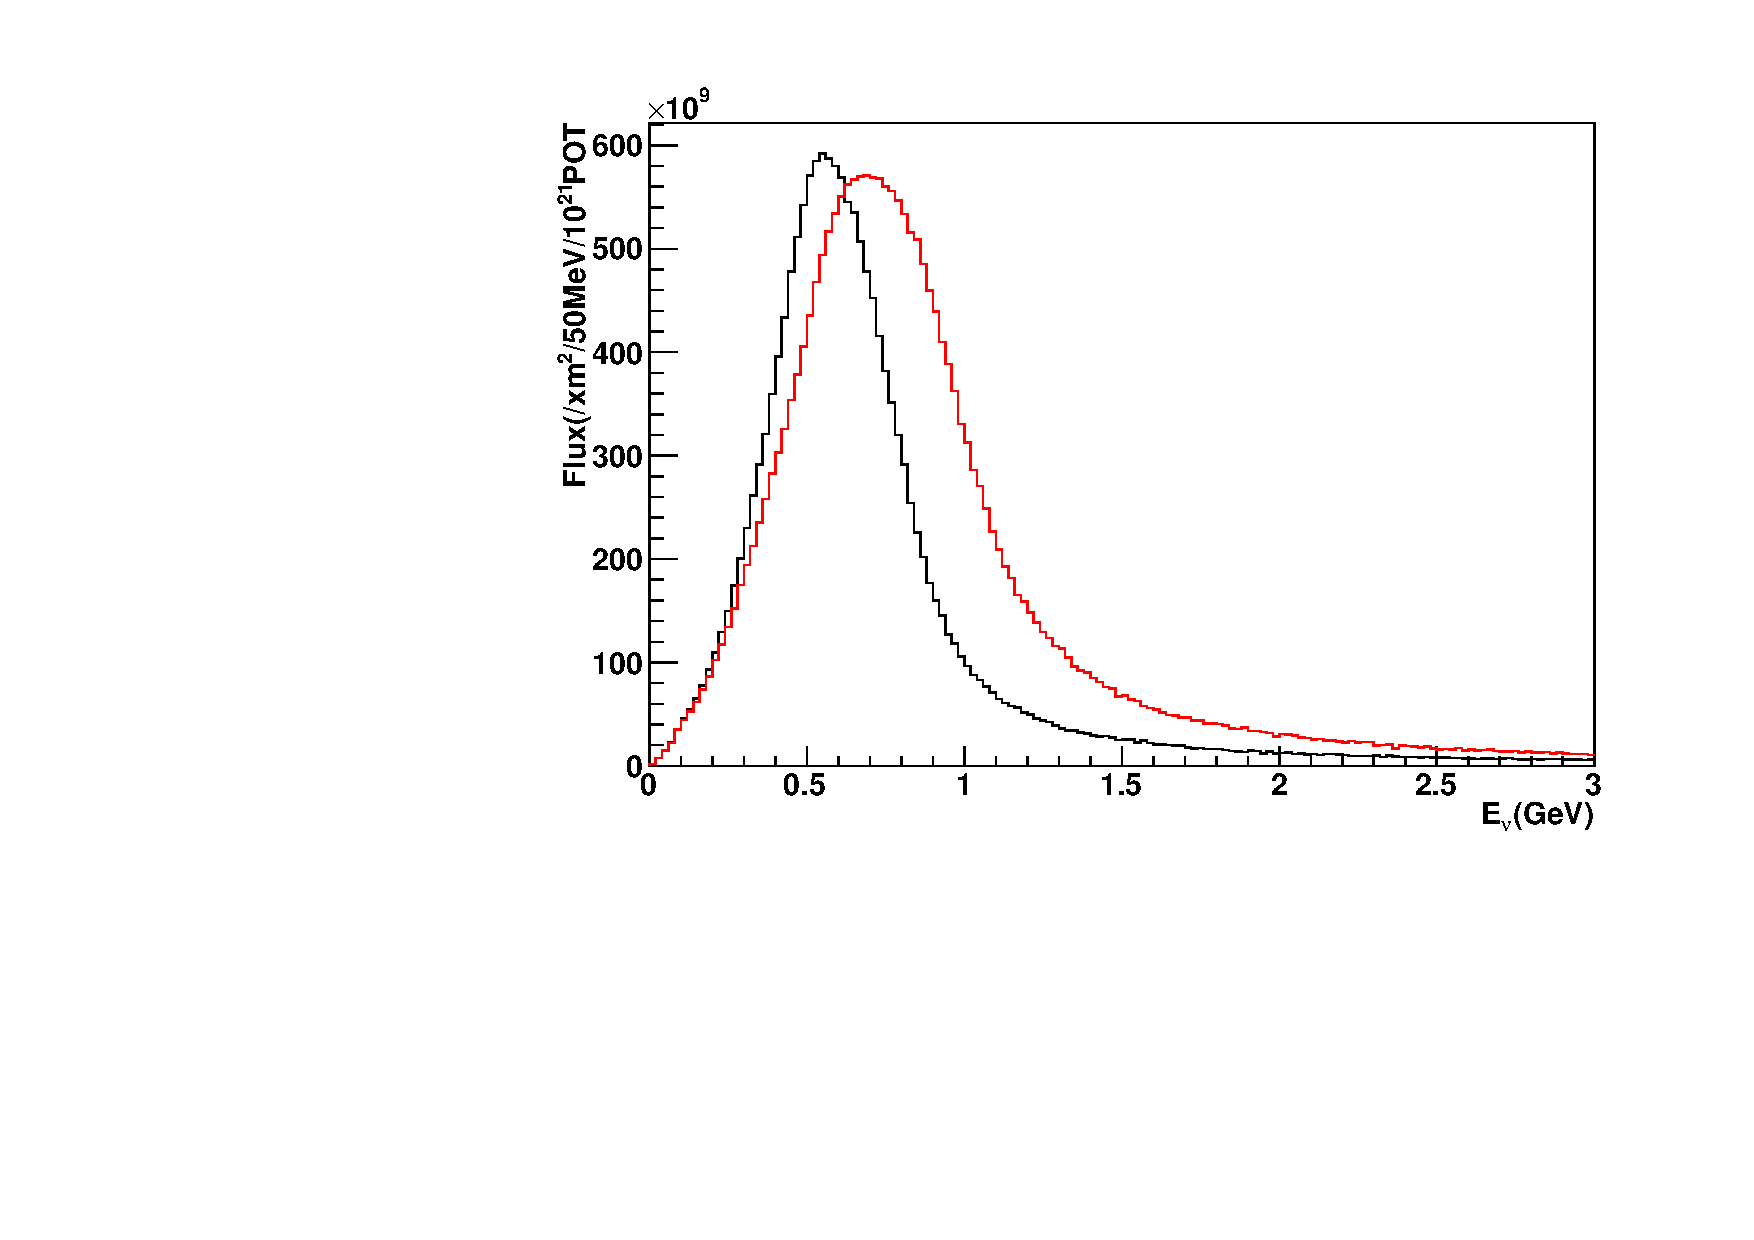
\includegraphics[width=0.6\linewidth, angle=270]{fig/b2_nd280_fluxes.pdf}
\end{center}
\caption{
Neutrino energy spectrum at the candidate detector position(red, off-axis 1.5 degree).
The spectrum at the ND280 site (black, off-axis 2.5 degree) is also shown.
}
\label{fig:b2flux}
\end{figure}

